% Figure 1: Main 3-Column Pipeline Architecture
% Design Spec: docs/era-smartfarm-rag/paper/figures/ARCHITECTURE_FIGURE_DESIGN.md
% TODO: Replace with actual TikZ diagram implementing full 3-column layout

\begin{figure}[htbp]
\centering
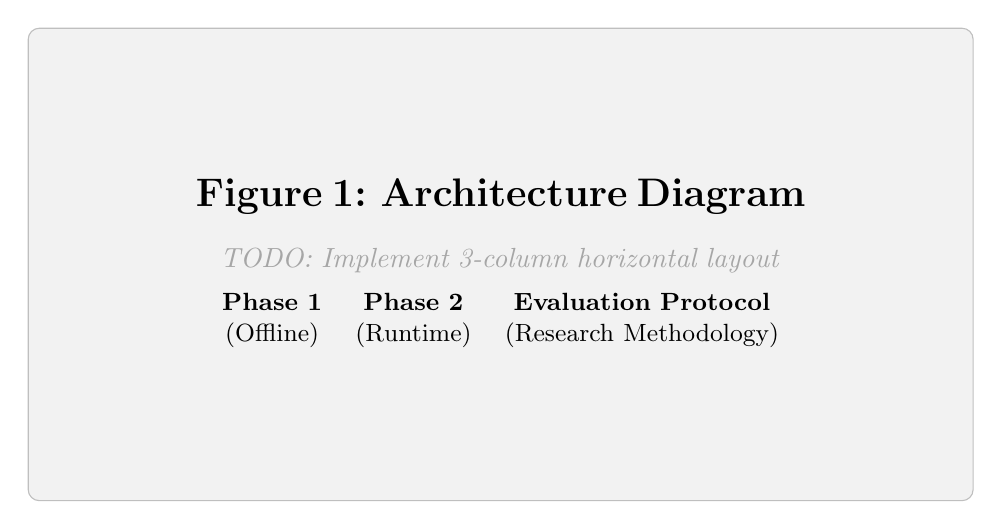
\begin{tikzpicture}
  \node[rectangle, draw=gray!50, fill=gray!10, minimum width=12cm, minimum height=6cm, rounded corners] (placeholder) {};
  \node[text width=10cm, align=center] at (placeholder.center) {
    \textbf{\Large Figure 1: Architecture Diagram}\\[1em]
    \textcolor{gray!70}{\textit{TODO: Implement 3-column horizontal layout}}\\[0.5em]
    \small
    \begin{tabular}{ccc}
    \textbf{Phase 1} & \textbf{Phase 2} & \textbf{Evaluation Protocol} \\
    (Offline) & (Runtime) & (Research Methodology) \\
    \end{tabular}
  };
\end{tikzpicture}
\caption{ERA-SmartFarm-RAG: End-to-End Research Pipeline with 3-column architecture showing Phase 1 (Data \& Index Build), Phase 2 (Runtime Inference with HybridDAT), and Evaluation Protocol (Dataset Generation + Metrics).}
\label{fig:architecture}
\end{figure}
